\subsection{Выбор микроконтроллера}

Так как автор курсовой работы уже имел опыт работы с МК производителя \textit{ST Microelectronics}, выбор существенно сузился. Однако у компании имеется довольно обширных выбор микроконтроллеров, которые разделяются на:
\begin{enumerate}
    \item Для беспроводных решений: STM32WB3 и STM32WL3
    \item Малопотребляющие:  STM32L0, STM32L1,  STM32L5, STM32L4 и STM32L4+
    \item Базовые характеристики: STM32F0, STM32G0, STM32F1, STM32F3 и STM32G4
    \item Высокая производительность: STM32F2, STM32F4, STM32F7 и STM32H7   
\end{enumerate}

На изображении \ref{fig:stm32_options} изображена диаграмма сфер использования микроконтроллеров компании \textit{ST Microelectronics} к линейке МК.
\begin{figure}[ht]
    \centering
    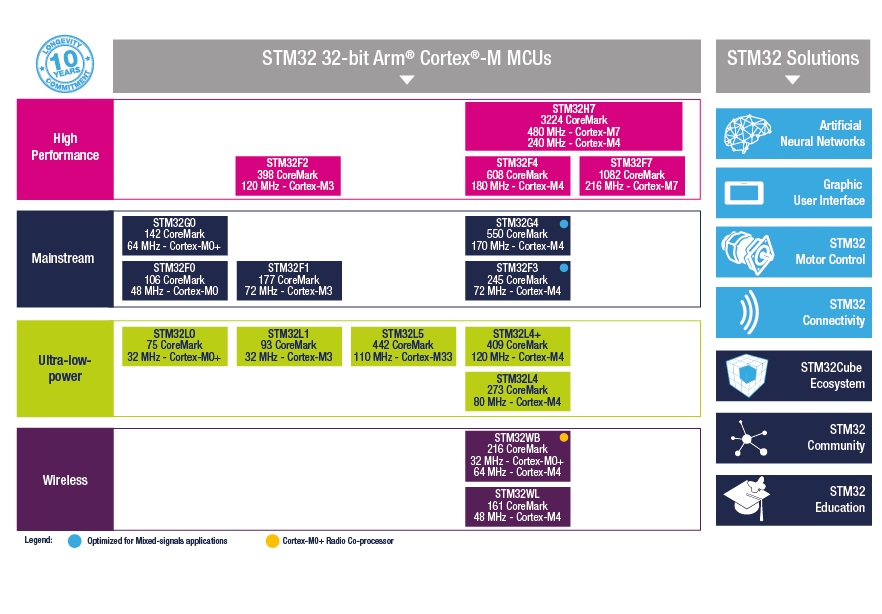
\includegraphics[width=0.85\linewidth]{\commonSecPathPrefix/sec_1/content/STM32_All.jpg}
    \caption{Линейка МК STM32}
    \label{fig:stm32_options}
\end{figure}

Проект \textit{"Эмулятор контроллера светодиодного экрана"} проектируется с учетом будущего апгрейда, соответственно важно предусмотреть возможность подключения внешних систем для взаимодействия с ними. Для этого будут использованы интерфейсы.

\subsubsection{Интерфейс}

Интерфейс - граница между двумя функциональными объектами, требования к которой определяются стандартом; совокупность средств, методов и правил взаимодействия (управления, контроля и т. д.).

На устройство будут вынесены следующие интерфейсы:
\begin{itemize}
    \item I2c
    \item UART
\end{itemize}

Для индикации работы устройства будет использован 1 \textit{RGB} светодиод. Для его управления необходимы таймеры, которые смогут генерировать сигнал Широтно-импульсной модуляции (ШИМ).

Для управлением самим субмодулем экрана необходимо выдавать сигнал на следующие линии:
\begin{itemize}
    \item R1-R3
    \item G1-G3
    \item B1-B3
    \item A,B,C,D,E
    \item OE
    \item CLK
\end{itemize}

В связи с этими требованиями был выбран микроконтроллер \textit{STM32F103RCT6}, имеющий следующие характеристики:
\begin{figure}[ht]
    \centering
    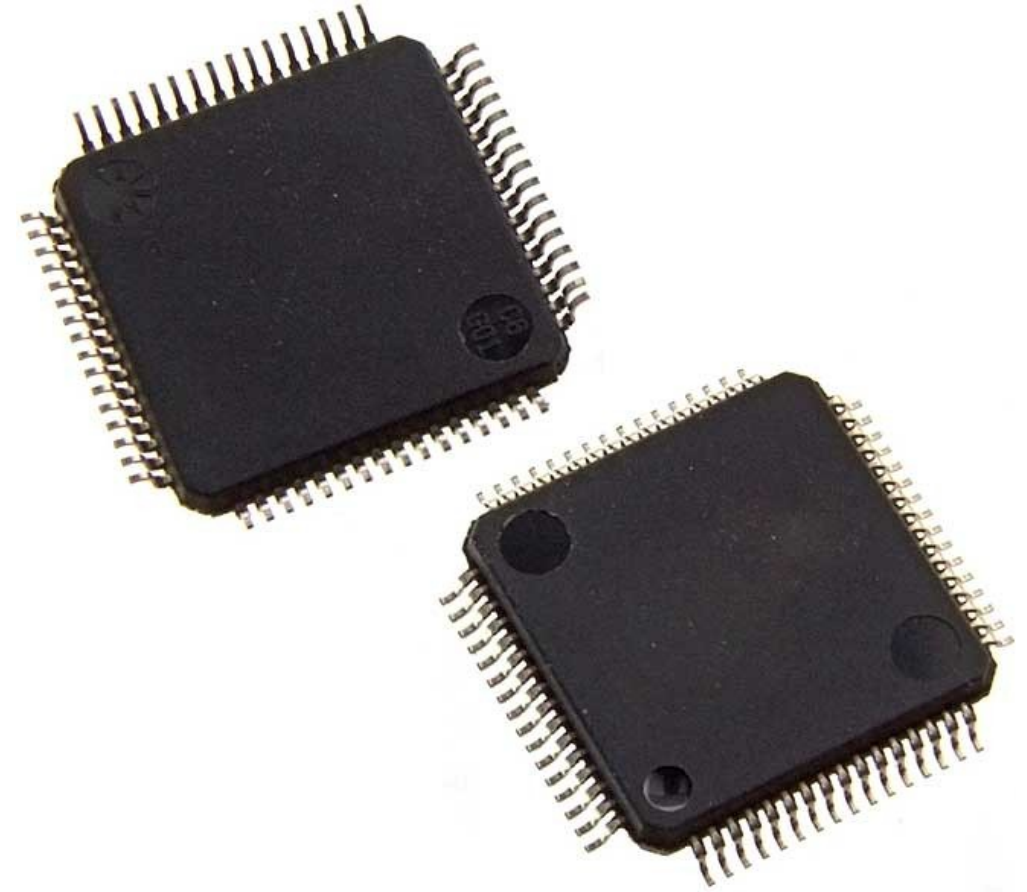
\includegraphics[width=0.6\linewidth]{\commonSecPathPrefix/sec_1/content/STM32F103RCT6.png}
    \caption{STM32F103RCT6}
    \label{fig:STM32F103RCT6}
\end{figure}

\begin{itemize}
    \item 3x SPI
    \item 2xI2S
    \item 2x I2C
    \item 5xUART
    \item USB
    \item CAN
    \item 8x таймеров
    \item 51 I/O
    \item 3xАЦП 16 каналов
    \item 2x ЦАП
    \item Тактовая частота - 72М Гц
    \item Объем памяти программ -  	256 КБайт
\end{itemize}

Выбор микроконтроллера STM32F103RCT6 вместо более современных альтернатив, таких как Atmel, ESP (Espressif Systems) или же Atmega, может быть объяснен несколькими факторами. Важно учитывать, что конечный выбор микроконтроллера зависит от конкретных требований проекта и ресурсов разработчика. Бюджетные ограничения: STM32F103RCT6 обычно доступен по более низкой цене по сравнению с некоторыми современными альтернативами. Производительность и ресурсы: STM32F103RCT6, несмотря на свои ограниченные ресурсы, может быть более чем достаточным для реализации базовой системы сигнализации. Если проект не требует сложной обработки данных или больших объемов памяти, то STM32F103RCT6 может обеспечить стабильную работу и долгий срок службы. 